\begin{enumerate}
 
 \item[a)] \texttt{Checking rules}: São regras de verificação que podem realizar uma busca no modelo à procura de padrões de erros conhecidos no código e relatá-los ao usuário, também são conhecidas como análise estática de código. O \gls{MPS} diferencia os problemas conforme a severidade: \textit{erros}, \textit{warning} e \textit{infos}, respectivamente, por meio de destaques nas cores vermelha, amarela e cinza;
 
 \item[b)]\texttt{Inference Rules}: Uma regra de inferência para um determinado \textit{concept} é responsável principalmente por computar um tipo para instâncias desse conceito. O \gls{MPS} fornece uma série de métodos de inferência, tais como: expressões de \textit{typeof}, declarações \textit{when concrete}, \textit{equations} e \textit{inequations}, etc. Esses recursos podem ser utilizados, por exemplo, para verificar se o tipo de uma variável local é igual ao tipo da sua declaração;
 
 \item[c)]\texttt{Quick Fix}: São responsáveis por implementar correções automáticas, fornecendo uma função de transformação do modelo, eliminando o problema relatado para o usuário. Por exemplo, um quick fix poderia ser criado para eliminar automaticamente trechos de código ou declarações duplicadas.
\end{enumerate}


A Tabela \ref{tblcheckingrules}, apresenta a lista de \texttt{checking rules} implementadas na DSL Cotas, enquanto a Tabela \ref{tblquickfixes}, elenca os elementos de \texttt{quick fixes} implementados como recursos de apoio ao usuário.

\newpage
\begin{table}[ht]
\caption{\textit{Checking rules} da DSL Cotas}
\label{tblcheckingrules}
\centering

\begin{tabular}{|p{6cm}|p{8cm}|}
\hline
\texttt{categoria\_resestante\_vagas} & Busca identificar se o último ramo de uma divisão de vagas é preenchida pelo usuário com a constante \texttt{RESTANTE\_VAGAS}.                                                                                      \\ \hline
\texttt{categoria\_unica} & Impede siglas de categorias de cotas duplicadas.                         \\ \hline
\texttt{codigo\_versao\_lei}          & Valida padrões de preenchimento dos dados de identificação da lei de cotas.                                       \\ \hline
\texttt{configuracao\_simples}          & Impede que o usuário preencha expressões complexas em uma definição do conceito \texttt{Configuracao}.
                        \\ \hline
\texttt{divisao\_pelo\_menos\_dois\_ramos}          & Garante que uma divisão de categoria possua pelo menos 2 (duas) categorias, exceto o ramo raiz.
                        \\ \hline
\texttt{filha\_sem\_reserva}          & Verifica se todas as categorias possuem o campo de percentual de reserva preenchido.

\\ \hline
               
\texttt{formato\_sigla\_cota}          & Faz o \textit{matching} da \texttt{String} de siglas de cota, permitindo apenas caracteres alfanuméricos maiúsculos.
\\ \hline

\texttt{distribuicao\_nome}          & Garante que o ramo raiz \texttt{TOTAL\_VAGAS} não tenha o nome alterado pelo usuário da DSL.
\\ \hline

\texttt{ordem\_prioridade\_duplicada}          & Valida se o usuário informou uma categoria de cota duplicada no conceito \texttt{OrdemPrioridadeCotas}.
\\ \hline

\texttt{ordem\_prioridade\_catfilhas}          & Gera um \textit{warning} para o usuário quando uma categoria não foi informada na seção \texttt{OrdemPrioridadeCotas}.
\\ \hline

\texttt{warning\_nm\_inic\_cota}          & Sugere um nome de preenchimento para a sigla de cota que inicie com o prefixo da cota anterior, por exemplo: a cota de estudantes de renda inferior (sigla RI), que fica dentro da categoria de escola pública (sigla EP), tem como sugestão EP\_RI, para facilitar a identificação.
\\ \hline

\end{tabular}

  \par\medskip\textbf{Fonte:} Elaborada pelo autor (2020). \par\medskip
\end{table}

\newpage
\begin{table}[ht]
\caption{\textit{Quick fixes da DSL Cotas}}
\label{tblquickfixes}
\centering

\begin{tabular}{|p{6cm}|p{9cm}|}
\hline
\texttt{preenche\_totalvagas\_name} & \textit{Quick fix} associado ao erro gerado pela \textit{checking rule} \texttt{distribuicao\_nome}, faz o preenchimento automático do nome padrão no ramo raiz de distribuição de vagas.                                                                                      \\ \hline
\texttt{remover\_categoria\_duplicada} & \textit{Quick fix} associado ao erro gerado pela \textit{checking rule} \texttt{categoria\_unica}, sugere a remoção automática do ramo de distribuição com a duplicidade.

\\ \hline
\texttt{reserva\_vagas\_ultima\_da\_lista} & \textit{Quick fix} associado ao erro gerado pela \textit{checking rule} \texttt{categoria\_resestante\_vagas}, sugere a correção automática da distribuição de vagas para preenchimento adequado da constante \texttt{RESTANTE\_VAGAS}.

\\ \hline
\texttt{sugere\_sigla\_nome} & \textit{Quick fix} associado ao \textit{warning} gerado pela \textit{checking rule} \texttt{warning\_nm\_inic\_cota}, sugerindo a correção automática para padronização do nome das siglas de distribuição.
                  \\ \hline      

\end{tabular}

  \par\medskip\textbf{Fonte:} Elaboração do autor (2020) \par\medskip
\end{table}




Com relação aos recursos de regras de inferência (\textit{inference rules}), foram definidas as regras: \texttt{typeof\_CategoriaCota} e \texttt{typeof\_Configuracao}, criadas para verificar se os valores dos percentuais são preenchidos somente com expressões ou referências do tipo \texttt{double}.

Por fim, as Figuras \ref{fig:checkingrule}, \ref{fig:quickfix} e \ref{fig:inferencerule}, demonstram exemplos de como foram implementadas, respectivamente, as \textit{checking rules}, as \textit{quick fixes} e as \textit{inference rules}. 
\begin{figure}[ht!]
\centering

\caption{\textmd{Exemplo de \textit{checking rule}}}
\label{fig:checkingrule}
\fcolorbox{gray}{white}{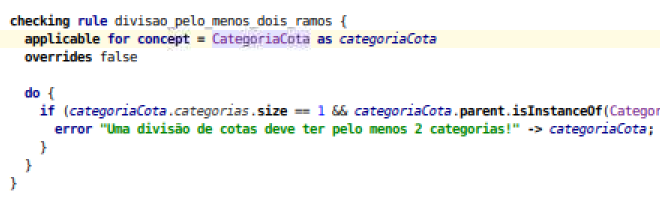
\includegraphics[width=0.85\textwidth]{chapters/dslcotas/mps/imagens/chekingrules.png}}

\par\medskip\textbf{Fonte:} Elaborada pelo autor (2020). \par\medskip

\end{figure}


\begin{figure}[ht!]
\centering

\caption{\textmd{Exemplo de \textit{quick fix}}}
\label{fig:quickfix}
\fcolorbox{gray}{white}{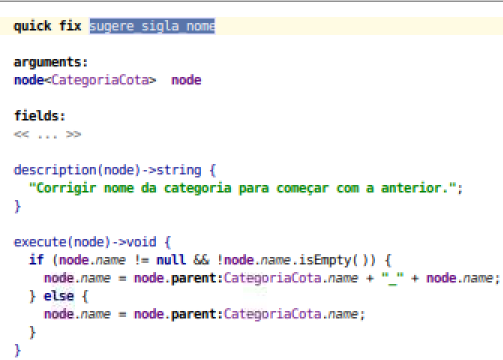
\includegraphics[width=0.85\textwidth]{chapters/dslcotas/mps/imagens/quickfixes.png}}

\par\medskip\textbf{Fonte:} Elaborada pelo autor (2020). \par\medskip

\end{figure}

\begin{figure}[ht!]
\centering

\caption{\textmd{Exemplo de \textit{inference rule}}}
\label{fig:inferencerule}
\fcolorbox{gray}{white}{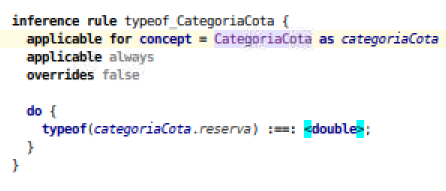
\includegraphics[width=0.85\textwidth]{chapters/dslcotas/mps/imagens/inferencerule.png}}

\par\medskip\textbf{Fonte:} Elaborada pelo autor (2020). \par\medskip

\end{figure}
